\documentclass[11pt]{article}
\usepackage[preprint]{acl}
\usepackage{times}
\usepackage[T1]{fontenc}
\usepackage[utf8]{inputenc}
\usepackage{graphicx}
\renewcommand{\ttdefault}{cmtt}

\newcommand{\mgd}{\textsc{mgd-hf}}
\newcommand{\ci}[2]{[#1,\,#2]}

\title{A Confirmed Pattern Without a Confirmed Cause:\\
Group Delay Dispersion Separates Synthetic Speech More in Sonorants,\\
and So Does a Resampler}

\author{Darwin Zhang}

\begin{document}
\maketitle

\begin{abstract}
We pre-registered and confirmed that the dispersion of Modified Group Delay over
the upper spectrum separates genuine from synthetic speech more strongly in
sonorants than in obstruents, relative to a cepstral statistic, on ASVspoof
2019 LA: a difference of $+0.063$ \ci{+0.045}{+0.080} in folded AUC. The natural
reading is a phase artifact of vocoding, concentrated where speech is periodic.
We then tried to break that reading, and it is not supported. A low quality sample
rate conversion applied to genuine speech, with no synthesis involved,
reproduces the pattern at full size. A magnitude statistic, spectral tilt,
tracks it. The pooled pattern survives resampling of utterances, speakers and
synthesis systems, and an identical low pass on both classes on the
evaluation partition; individual systems vary, and one reverses. We report it as a confirmed observation whose cause is
undecided, and describe the checks that changed our own conclusion.
\end{abstract}

\section{Introduction}

Detectors for synthetic speech are strong \citep{jung2022aasist}, and say little
about where in speech their evidence lies. A complementary question is
descriptive: is the difference between genuine and synthetic speech spread
evenly across classes of sound? If a vocoder must reconstruct harmonic phase,
one would expect an artifact where speech is voiced and periodic, and little
where it is noise-like.

We test the pattern that idea predicts with one fixed pair of statistics, under
pre-registration, and then subject the result to the checks a sceptic would
ask for. This paper is mostly about those checks. Separations here run from
0.51 to 0.60 AUC. Nothing in it is a detector.

\section{Method}

\paragraph{Data.} ASVspoof 2019 Logical Access \citep{wang2020asvspoof}. The
evaluation partition supplies 1,500 bonafide utterances from 67 speakers and
115 utterances from each of 13 synthesis systems, A07 to A19. The development
partition, with systems A01 to A06, is used only for a second registered test.

\paragraph{Segmentation.} A multilingual phone recogniser
\citep{xu2022zeroshot} gives a frame-level phone sequence. Each run of a phone
becomes a slice, assigned to one of six categories: nasals, approximants and
steady vowels (sonorants), and fricatives, plosives and affricates
(obstruents). This yields 64,693 slices on the evaluation partition, and 4,303 more of
diphthongs, which are not in the test. The
segmentation is approximate: 89\% of slices are a single 20\,ms frame widened
to a 60\,ms floor.

\paragraph{Statistics.} The phase statistic, \mgd, is the standard deviation of
Modified Group Delay \citep{murthy2003mgd} over the upper half of the spectrum,
4 to 8\,kHz. The magnitude statistic is the spread of MFCC frames within the
slice. Both were fixed before the evaluation data was examined.

\paragraph{Quantities.} For a statistic and a category, separation is the
folded AUC, $|\mathrm{AUC}-0.5|+0.5$. The \emph{advantage} in a category is the
separation of \mgd{} minus that of the magnitude statistic. The \emph{level} is
the mean advantage over the three sonorant categories. The \emph{asymmetry} is
the level minus the mean advantage over the three obstruent categories. The
registered hypothesis, H1, is that the asymmetry is positive with a 95\%
interval excluding zero.

\paragraph{Inference.} Slices are not independent, so intervals come from a
cluster bootstrap \citep{efron1993bootstrap} with 2,000 draws in which one
resample of clusters serves every category in a draw. The registered cluster
is the source utterance. A percentile bound is itself an estimate, so each
bound carries a distribution-free Monte Carlo band, and a verdict that turns on
a bound inside that band is reported as undecided.

\section{The confirmed pattern}

\begin{figure}[t]
\centering
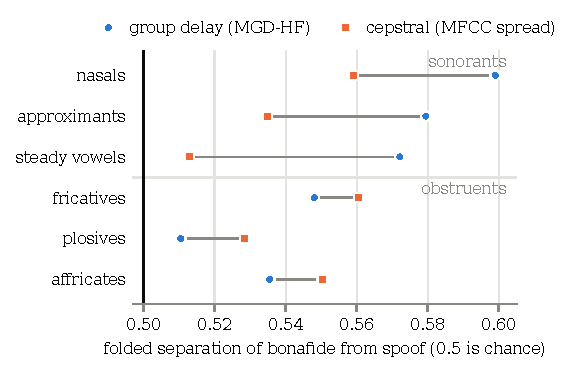
\includegraphics[width=\columnwidth]{figures/separation.pdf}
\caption{Separation of bonafide from spoofed speech by category, evaluation
partition. The group delay statistic leads in sonorants and not in
obstruents.}
\label{fig:separation}
\end{figure}

Figure~\ref{fig:separation} shows the pattern. The level is $+0.048$
\ci{+0.035}{+0.061} and the asymmetry $+0.063$ \ci{+0.045}{+0.080}. All
registered falsification conditions were decided in favour of H1.

\section{How far it reaches}

\begin{figure}[t]
\centering
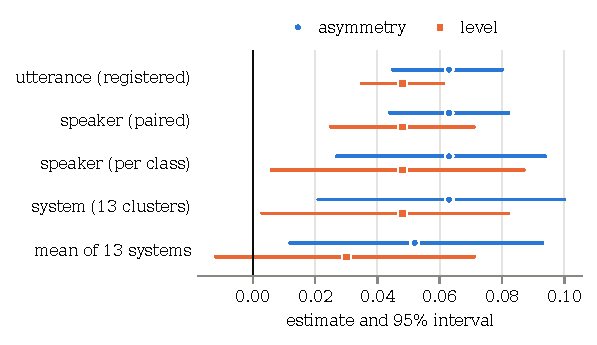
\includegraphics[width=\columnwidth]{figures/clustering.pdf}
\caption{The same two quantities under different choices of what the bootstrap
resamples, and as a mean over the 13 systems scored one at a time.}
\label{fig:clustering}
\end{figure}

\paragraph{What is resampled.} Clustering by utterance describes more
utterances from the same speakers and systems. Figure~\ref{fig:clustering}
asks more. The asymmetry excludes zero whether speakers or synthesis systems
are resampled. The level does not: with 13 system clusters its lower bound
sits on zero, and scored one system at a time its mean is $+0.029$
\ci{-0.012}{+0.071}. The pooled level is larger than that mean. The magnitude
statistic runs in different directions on different systems, which cancels in
a pool; how much of the gap that explains was not measured. System by system
the asymmetry is clearly positive on 4 of 13, clearly negative on one (A19)
and undecided on 8. A registered account of that variation, that it follows
whether a system generates or inherits its waveform phase (H3), held in
direction on all six development systems but is not supported: pooled over
both partitions $p = 0.021$, and with algorithms present in both counted once,
$p = 0.16$.

\begin{figure}[t]
\centering
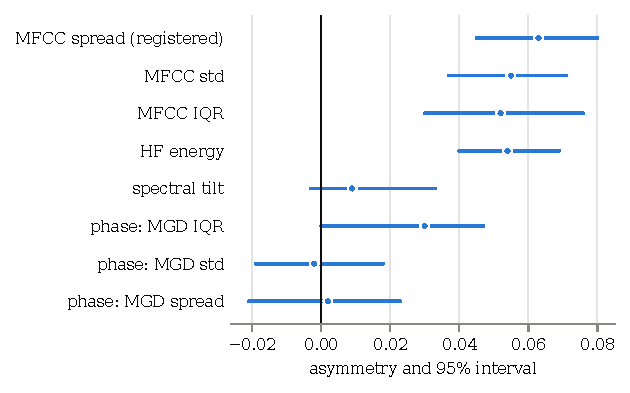
\includegraphics[width=\columnwidth]{figures/pair.pdf}
\caption{The asymmetry under other pairs of statistics. The first five rows
keep \mgd{} and change the magnitude comparator. The last three keep the
registered comparator and change the phase statistic to a whole-band one. It
holds against cepstral and energy statistics and vanishes against spectral
tilt.}
\label{fig:pair}
\end{figure}

\paragraph{Which statistics.} Figure~\ref{fig:pair} swaps one side of the pair
at a time. These are sensitivity analyses on data already seen, not tests. Two
things follow. The asymmetry belongs to upper-band group delay dispersion, not
to phase statistics in general. And with spectral tilt as the comparator it is
$+0.009$ \ci{-0.003}{+0.033}: a magnitude statistic with no phase content shows
nearly the same sonorant-over-obstruent pattern.

\section{Is it synthesis at all?}

\begin{figure}[t]
\centering
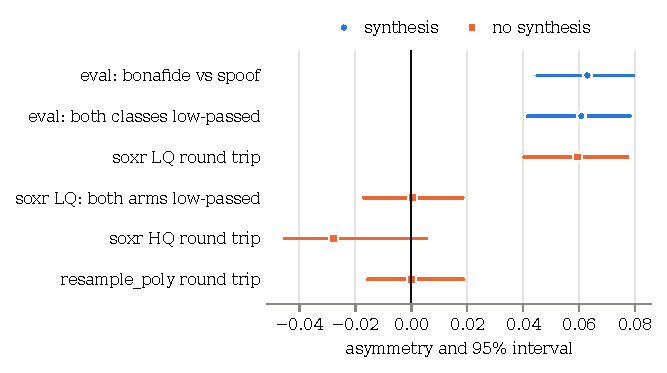
\includegraphics[width=\columnwidth]{figures/resampler.pdf}
\caption{Asymmetry for the real comparison and for genuine speech against the
same speech after a 16 to 22.05 to 16\,kHz round trip. One resampler reproduces
the effect with no synthesis. An identical low pass removes that artifact and
leaves the real one.}
\label{fig:resampler}
\end{figure}

An anti-alias filter would be expected to change group delay near the band
edge, which is what \mgd{} reads. We wrote three decision rules before
reading any audio, though they entered the repository with the results, then
compared each bonafide utterance with itself after a sample rate round trip,
rounded back to 16 bit (Figure~\ref{fig:resampler}).

With a low quality resampler, whose passband rolls off from about 6\,kHz, the
asymmetry is $+0.059$ \ci{+0.040}{+0.077} and the level $+0.055$: the size,
direction and category order of the real result. Two sharper resamplers do not
reproduce it: one gives $+0.000$ and the other $-0.028$, the opposite sign. So the signature of H1 is not specific to synthesis, and the rule
written to detect that fires.

The same artifact is nonetheless not what the corpus shows. One identical
linear-phase low pass at 6.9\,kHz on both arms takes the planted asymmetry to
$+0.001$ \ci{-0.017}{+0.018}, and leaves the real one at $+0.061$
\ci{+0.042}{+0.078}. The low pass cannot rule out a difference in spectral
shape below its cutoff, and the tilt result suggests there is one.

\begin{figure}[t]
\centering
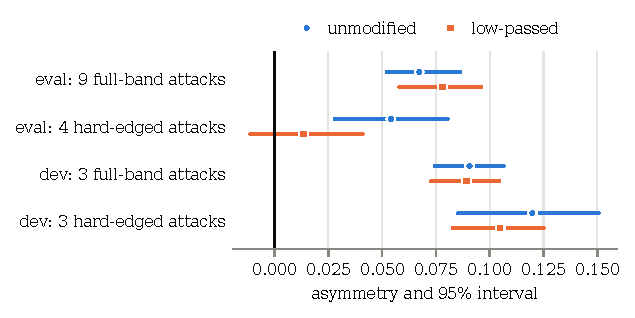
\includegraphics[width=\columnwidth]{figures/split.pdf}
\caption{A split seen after the fact on the evaluation partition, and its
registered test on the development partition, where it does not replicate.}
\label{fig:split}
\end{figure}

\paragraph{A post hoc split, tested.} Four evaluation systems carry a hard band
edge near 7.7\,kHz, and pooled over them the asymmetry did not survive the low
pass (Figure~\ref{fig:split}). Because that split was chosen after seeing the
data, we registered it and tested it on the development partition before
reading its audio. Three of its six systems are hard-edged. Pooled over those
three the asymmetry is $+0.105$ \ci{+0.083}{+0.125} after the low pass, so the
split does not replicate. An independent re-derivation reproduced these numbers
and narrowed their reading: the pool is positive only because of one system
(A01), the other two have a negative asymmetry that the low pass moves toward
zero, and over all six systems the low pass lowers the asymmetry by $0.033$
\ci{0.027}{0.039}. On this partition the low pass is not inert; which attacks move, and in
which direction, is not settled by three against three. The pooled
prediction about them failed.

\section{What we got wrong}

Four errors were caught by re-derivation rather than by review of our own
reasoning, and each changed a published number or sentence.
(i) Intervals on the level were first computed by resampling each category
independently, which ignores that one utterance feeds all three; they were
about 30\% too narrow.
(ii) Under system clustering the printed verdict changed with the random seed.
(iii) The registered primary test, the interval on the asymmetry, was printed
but not used in the verdict.
(iv) We first set aside the one resampler that reproduces the effect, on the
ground that it also moves the magnitude statistic, which the real comparison
does too.

\section{Limitations}

One corpus and one language. Thirteen systems and 67 speakers. Percentile
intervals, which cover less than their nominal rate with 13 clusters. A
segmentation that is close to fixed windows. The development result was
re-derived independently once; the size of the change under the low pass
depends on the filter cutoff and on whether affricates are counted. The statistic pair was
chosen on an earlier partition as the strongest of several, and the result is
specific to it.

\section{Conclusion}

The pattern is real in the sense that matters for a registered claim: it was
predicted, it appeared, and it survives changes of resampling unit, an
equalising low pass and a second partition. Its interpretation as a phase
artifact of synthesis is not supported. A resampler produces the same
signature, and spectral tilt carries the same pattern. A control in which
magnitude is real and phase is wholly synthetic is registered and not yet run;
it is the test that can separate the two accounts.

\section*{Reproducibility}

Code, the slice tables, registrations and the commands behind every number are
in the project repository. Figures are drawn by
\texttt{scripts/make\_report\_figures.py}. The detailed records are
\texttt{docs/ROBUSTNESS.md}, \texttt{docs/BAND-EDGE.md} and the registration
documents.

\bibliography{references}

\end{document}
